
\section{Introduction}

In \field, various procedures use the same few atomic operations. For instance, accessing the neighbours of a given node is key to a wide range of problems such as computing shortest paths, finding connected components, detecting communities etc. Making this type of elementary operation faster would improve such algorithms without having to modify their implementation \cite{gorder}.
Cache optimisation can have that effect: if two variables are often accessed together by algorithms, they should be stored side-by-side in memory so that they are copied together on a cache line. In a graph, it means reordering the nodes so that neighbours have close-enough indices. A cache-miss happens when data is not available in cache. The processor then has to fetch it in main memory, which is up to twenty times slower, depending on the machine architecture. As this cache stall is known to represent a significant share of the computation time \cite{cache,cache2}, reducing it can lead to important speedups.

This work replicates~\cite{gorder} by Hao Wei \textit{et al.} which introduces Gorder, a new procedure to order nodes in a graph, and compares it to other standard orderings using typical algorithms and datasets as benchmarks. Because of the variety of graph algorithms, it is impossible to find an ideal ordering, which makes it interesting to propose and compare different strategies. The authors of the original paper claim an improvement of 10 to 50\% in \runtime, due to lower cache-miss rate.

We were able to replicate most of the experiments and confirm that ordering nodes according to Gorder makes the implementations 10 to 50\% faster than without ordering.
%
Section~\ref{method} presents the algorithms, orderings and datasets as well as issues faced during the replication. Our results are presented in Section~\ref{results} and are compared to the original results. Finally, Section~\ref{discussion} discusses the relevance of such an ordering compared to simpler ordering methods that offer satisfactory performances.

\begin{figure}%[h]
\begin{subfigure}{0.49\textwidth}
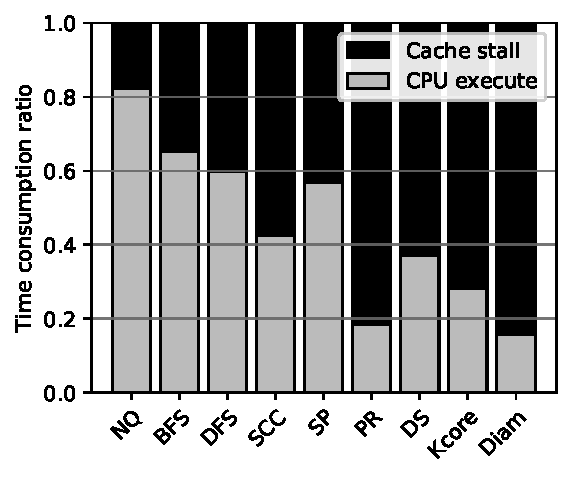
\includegraphics[width=\linewidth, height=5cm]{img/img-cache-original.pdf} 
\caption{Original order}
\label{img-cache-original}
\end{subfigure}
\begin{subfigure}{0.49\textwidth}
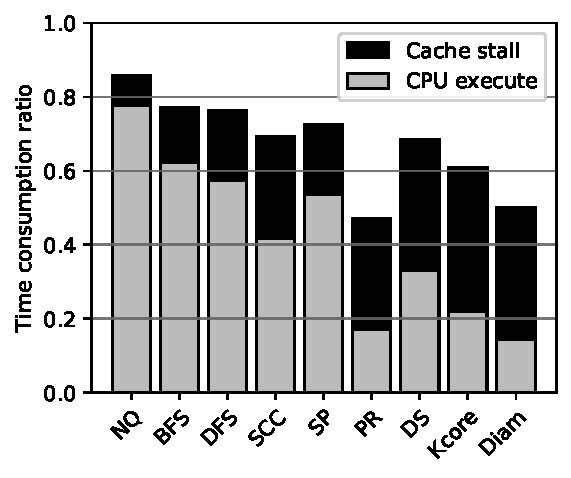
\includegraphics[width=\linewidth, height=5cm]{img/img-cache-gorder.pdf}
\caption{Gorder}
\label{img-cache-gorder}
\end{subfigure}
\caption{\textbf{CPU execution and cache stall.} Original order and Gorder are compared for all algorithms on \textit{sdarc} dataset. Grey bars are time spent on CPU operations, black bars represent time spent waiting for data retrieval. Figure~(a) shows the normalised \runtime s with the original order, figure~(b) shows the \runtime s when the network has been reordered following the Gorder procedure. While both need about the same CPU time, the latter is significantly faster due to cache stall reduction. Compare to Figure~1 in~\cite{gorder}.}
\label{img-cache}
\end{figure}


\section{Method} \label{method}

The original study~\cite{gorder} was motivated by the observation that cache stall can take up to 70\% of the whole computation time, which is supported by the observations reported in Figure~\ref{img-cache}.
%
 This issue has been addressed for specific algorithms such as breadth-first search~\cite{bfs-cache}.
 In~\cite{gorder}, the authors use a more general method: they reorganise the data to draw more benefit from the cache system, regardless of the algorithm or of the exact hardware specifications.
 

 Gorder clusters nodes that are likely to be accessed simultaneously by any graph algorithm.
 %
 More precisely, let us consider a graph $G=(V,E)$ with $n=|V|$ nodes and $m=|E|$ edges. The proximity of two nodes $u$ and $v$ is measured by a score $S(u,v)$ which increases if they are neighbours and if they share many common in‐neighbours.
 %
 The total score $F$ is the sum of $S(u,v)$ for all nodes $u$ and $v$ that have close indices. 
 %
 Window size $w$ is the parameter that defines this closeness.
 %
 Gorder creates an arrangement $\pi$ of the indices to maximise $F$. 
  %
 We note $\pi_u$ the index of a node $u$ in such an arrangement.
 %
 We give a more formal definition in Section~\ref{orders}.



 The authors prove that finding the optimal ordering $\pi$ is a NP-hard problem and propose a heuristic method with a theoretical approximation bound. % consequently
%
 They also present practical optimisations to reduce its time complexity. 
 Finally, they run extensive experiments to compare their order to other standard orders. 

Although the theoretical results of the original paper are important to explain the efficiency of Gorder, we only focus here on the algorithms and experiments. They provide an extensive analysis by comparing the \runtime s for nine typical algorithms on eight large datasets with nine possible orderings. The current section describes them all and presents the replication issues that they imply. It also details the data structures that we used in this project. All the codes and instructions for this purpose can be found in our repository\footnote{\url{https://github.com/lecfab/rescience-gorder}}.



%%%%%%%%%%%%%% ALGORITHMS

\subsection{Algorithms} \label{algorithms}

The original paper selects typical graph algorithms to test the different orderings. 
%
As implementation details are not fully documented and as its authors were not able to provide answers to some of our questions on this topic, we list below the details of our implementations.


\subsubsection{Neighbour query (NQ)}

Listing the neighbours of a given node is a standard elementary operation in \field.
%
As defined in~\cite{gorder}, this operation must \textit{access the out-neighbours} of each node. To ensure that neighbours are put in cache, thus benefiting from a wise node ordering, an arbitrary operation is made over the set of neighbours. We compute for each node $u$ the sum of degrees of its neighbours:
$q_u=\sum_{v\in N_u} d_v$.

\subsubsection{Breadth and Depth-first search (BFS, DFS)}
BFS and DFS are standard graph traversal algorithms~\cite{cormen}. We adapted them to the data structure detailed in Section~\ref{datasets}. Note that neighbours are selected in lexicographic order.

\subsubsection{Strongly connected components (SCC)}
To cluster nodes of the graph that can be accessed from one another, we use \tarjan~\cite{tarjan}, which is a based on DFS.

\subsubsection{Shortest paths (SP)}
As in the original paper, we use \bellman~\cite{cormen} to compute the minimum distance from a source node to any other node. The time complexity after simple optimisations is in $O(\Delta m)$ where $\Delta$ is the diameter of the graph and $m$ is the number of edges. 
%
As real-world networks are known to have relatively small diameters ($\Delta \ll n$), this algorithm works on massive datasets (see section~\ref{datasets}). 
%
Note that for unweighted graphs, shortest paths can be computed in linear time and space using a BFS, but we keep the algorithm suggested in~\cite{gorder} for comparison purposes.

\subsubsection{Page rank (PR)}
This is the algorithm presented in~\cite{pagerank} to rank webpages. It gives a score to each node according to its importance in the network structure.
%
The original paper hints at an approximation based on the power iteration method with 100 iterations. We implement it with a damping factor set to $\alpha=0.85$ which is a usual configuration.


\subsubsection{Dominating set (DS)}
A dominating set is a subset of nodes such that every node of the graph either belongs to the subset or has a neighbour in it. The implementation is not described in the original paper so we use a greedy approximation~\cite{cormen}: first, we select the node with the most uncovered neighbours and add it to the dominating set. Second, this node and all its neighbours are removed from the graph because they are now covered. The two steps are then repeated among the remaining nodes.

\subsubsection{Core decomposition (Kcore)}
This graph pealing algorithm~\cite{kcore} recursively removes the node of smallest degree until only a core of well-connected nodes remains. We use a binary heap structure to keep track of the degrees, leading to a quasi-linear time complexity.

\subsubsection{Diameter (Diam)}
Efficient approximations with theoretical bounds exist~\cite{BFSdiameter} to compute the aforementioned diameter $\Delta$. In~\cite{gorder}, the authors run 5000 times the shortest paths algorithm SP from a random node, and output the highest distance obtained. 
%
Note that the accuracy and efficiency of the algorithm are not key here, as the aim is to compare the performances in terms of computation time of different orderings.




%%%%%%%%%%%%%% DATASETS

\subsection{Datasets and data structure} \label{datasets}


\subsubsection{Size}
Eight real-world datasets are used as benchmarks in the original work~\cite{gorder}. Their basic features are reported in Table~\ref{table-datasets}.
%
As per usual with real-world graphs~\cite{networkProperties}, these graphs are sparse ($m \ll n^2$) and have small diameter and a skewed degree distribution, etc.
%
As shown in Table~\ref{table-datasets}, their sizes range from 1.6 million nodes and 30 million edges to almost 100 million nodes and two billion edges.
%
In order to facilitate further experiments, we attach the \textit{epinion} dataset to the repository, a smaller network on which our code can be tested quickly.



\subsubsection{Sources}
In the original paper, the sources are provided in the form of URLs where datasets can be downloaded. These data are available with the links given in Table~\ref{table-datasets}.
%, there is now a fee to access data from the Konect project.


\subsubsection{Categories}
The authors of~\cite{gorder} selected two main categories of real-world networks: online social platforms, where a node is a user and a directed edge represents a social interaction, and web graphs, where a node is a web page and an edge is a hyperlink.

\begin{table}[]
\centering
\begin{tabular}{r||c|c|c|c|c}
  %\hline
  Dataset & Size (Go) & Nodes (10$^6$) & Edges  (10$^6$) & Source & Category\\
  \hline%\hline
  \textit{pokec} & 0.4 & 1.63 & 30.6 & SNAP\textsuperscript{1} & Social \\
  \textit{flickr} & 0.4 & 2.30 & 33.1 & Konect\textsuperscript{2} & Social \\
  \textit{livejournal} & 1.0 & 4.85 & 69.0 & SNAP\textsuperscript{1} & Social \\
  \textit{wiki} & 6.7 & 13.6 & 437 & Konect\textsuperscript{2} & Web \\
  \textit{gplus} & 7.3 & 28.9 & 463 & Gong\textsuperscript{3} & Social \\
  \textit{pldarc} & 10 & 42.9 & 623 & WDC\textsuperscript{4} & Web\\
  \textit{twitter} & 26 & 61.6 & 1470 & Kaist\textsuperscript{5} & Social\\
  \textit{sdarc} & 34 & 94.9 & 1940 & WDC\textsuperscript{4} & Web \\
  \hline
  \parbox{1.6cm}{\hfill \textit{epinion}\\\null\hfill (added)} & 0.005 & 0.0759 & 0.509 & SNAP\textsuperscript{1} & Social \\
  %\hline
\end{tabular}
\caption{\textbf{General features of the datasets used in the experiments.} The data can be found in the following websites:\\
 \footnotesize{
   \textsuperscript{1}Stanford Network Analysis Project: \url{http://snap.stanford.edu/data/}\\
   \textsuperscript{2}Koblenz Network Collection: \url{http://konect.cc/networks/flickr-growth/} and \url{http://konect.cc/networks/wikipedia_link_en/}\\
   \textsuperscript{3}Gong Research Group: \url{http://gonglab.pratt.duke.edu/google-dataset}\\
   \textsuperscript{4}Web Data Commons: \url{http://webdatacommons.org/hyperlinkgraph/2012-08/download.html}\\
   \textsuperscript{5}Kaist Advanced Networking Laboratory: \url{http://an.kaist.ac.kr/traces/WWW2010.html}
 }
}
\label{table-datasets}
\end{table}

\subsubsection{Format}
The datasets are directed graphs given as lists of edges.
Most algorithms (\textit{e.g.} computing shortest paths) have different results depending on whether edges are directed or not.
%
In order to store large graphs in main memory, an efficient data structure is needed. 
%
Libraries exist for that purpose, but we develop our own light structure to have better control over the implementation of the algorithms.
%
A list of edges does not provide quick access to the list of neighbours of a given node, which is the crucial operation for most of the above graph algorithms. The data is therefore converted into an adjacency list, where a node points to the list of its neighbours. To store it efficiently, we use a \textit{Compressed Sparse Row} format, as described in Figure~\ref{img-format}.

\begin{figure}[h]
    \centering 
    \begin{subfigure}{0.25\textwidth}
        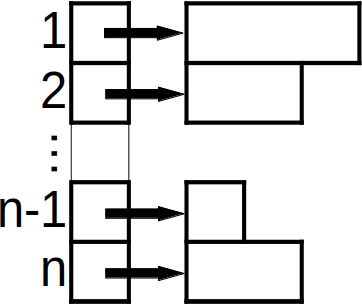
\includegraphics[width=\linewidth]{img/format-adjlist.png}
        \caption{Adjacency list}\label{img-format-adjlist}
    \end{subfigure}\hspace{0.05\textwidth}
    \begin{subfigure}{0.5\textwidth}
        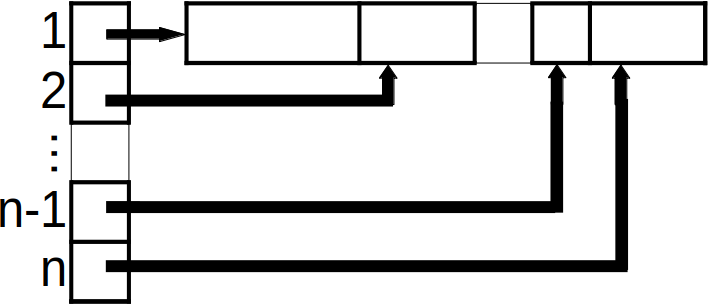
\includegraphics[width=\linewidth]{img/format-csr.png}
        \caption{Compressed Sparse Row}\label{img-format-crf}
    \end{subfigure}
    \caption{\textbf{Graph representations.} An adjacency list stores a list of neighbours for each node. In CSR, all the neighbours are stored in a shared array of size $m$, and each node has a pointer to its first neighbour. This is an equivalent but more compact format which allows for faster memory access. }\label{img-format}
\end{figure}



%%%%%%%%%%%%%% ORDERINGS

\subsection{Orderings} \label{orders}

We list below the different ordering methods considered in the original study and used as a benchmark for comparison with Gorder.

\subsubsection{Original}
Datasets are collected in a way that is not random but is rarely reported.
%
As shown in Section~\ref{results}, the original orderings perform quite well regarding cache miss.

\subsubsection{Random (added)}
In comparison to~\cite{gorder}, we added a random ordering, obtained by shuffling the indices of nodes.
%
We use it as a non-favourable benchmark for comparison to all other orderings. 

\begin{figure}[]
    \centering
    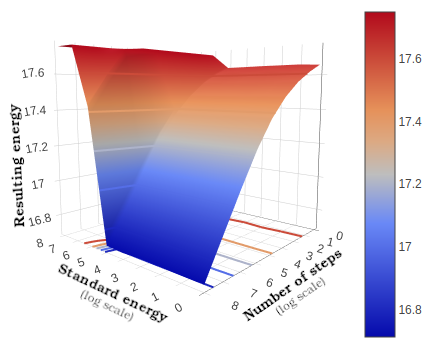
\includegraphics[width=.6\linewidth]{img/tune_sa.png}
    \caption{\textbf{Tuning simulated annealing.} The colour represents the energy of the best permutation $\pi$ obtained for various parameters on \textit{epinion}. Number of steps $S$ ranges from  $n$ to $m\log n$ (logarithmic scale), which we consider to be the maximal acceptable time for the heuristic implementation. Standard energy $k$ ranges from $1/(mn)$ to $mn$ (logarithmic scale). We observe that a) the higher $S$, the lower the resulting energy, b) when $k$ is high, the resulting energy is at a maximum: all swaps are accepted regardless of their quality which results in a random arrangement, c) any low value of $k$ has the same result, in particular for $k=0$ which corresponds to a local search.}\label{img-tune-sa}
\end{figure}


\subsubsection{MinLA and MinLogA} These acronyms stand for \textit{minimum linear} (respectively \textit{logarithmic}) \textit{arrangement}. The goal is to find an arrangement $\pi$ of the nodes that minimises a given ``energy" function. The energy $\mathcal{E}$ is computed over the set $E$ of edges in the following way:
$$\mathcal{E}_{MinLA}=\sum_{(u,v)\in E} |\pi_u-\pi_v|
\qquad\text{ and }\qquad
\mathcal{E}_{MinLogA}=\sum_{(u,v)\in E} \log|\pi_u-\pi_v|$$
%
As both exact optimisations are NP-hard, a heuristic method is necessary. The authors of~\cite{gorder} use simulated annealing: random permutations are achieved to decrease the energy $\mathcal{E}$, while the temperature goes down which allows less and less modifications. 
%
Simulated annealing is known to be hard to tune. Our implementation has two parameters: the number of steps $S$
%(how many random swaps are performed before stopping) 
and the standard energy $k$.
%(what typical tolerance is given to bad swaps).
%
The temperature $T$ decreases linearly so that, at step $s$, $$T(s) = 1 - s/S$$
%
At each step, two nodes are picked at random. Swapping their indices in $\pi$ leads to a variation $e$ of the total energy $\mathcal{E}$. If $e$ is negative, the swap is registered. Otherwise, it is registered with a probability $p$, inspired by statistical physics:
$$p(e,T)=\exp\left(-\frac{e}{k\cdot T}\right)$$

 In Figure~\ref{img-tune-sa} we test a wide range of values of $S$ and $k$ on \textit{epinion}. 
 %
 While we cover a significant fraction of the parameter space,  we are not able to find a combination of $S$ and $k$ that outperforms a simple local search ($k=0,p=0$), where only the favourable swaps are accepted. Below, we set $S=m$ and $k=m/n$.
 


\subsubsection{RCM}
The Reverse Cuthill–McKee ordering \cite{rcm} is a Breadth-First Search where nodes of small degree are favoured. It is meant to find an arrangement $\pi$ that reduces the bandwidth of a sparse graph, given by $\max_{(u,v)\in E} |\pi_u-\pi_v|$ with $ \pi_u $ the index of node $u$.

\subsubsection{Degsort} 
As proposed in the original paper, nodes are sorted in descending order of in-going degree.


\subsubsection{Chdfs}
We assume that the \textit{children-depth first search traversal} mentioned in~\cite{gorder} is a usual Depth-First Search algorithm. The first node is chosen at random, then the selection of children is made following the original order of node indices.

\subsubsection{SlashBurn (simplified)} 
%
SlashBurn is an iterative process that separates hubs (high-degree nodes) from low-degree nodes connected to hubs.
%
It creates an ordering by iterating over an array of size $n$, initially empty.
%
Each iteration divides the array in parts A, B and C. Part A takes only one node, selected at random among those with highest degree. All isolated nodes go to part C. Then these nodes are removed from the graph which creates new isolated nodes, and degrees are updated. Part B is filled by the next iteration until no node remains.

The original SlashBurn algorithm~\cite{slashburn} fills part C with disconnected components instead of isolated nodes and puts $r$ hubs in part A, where $r$ is a parameter. As no precise information was given in \cite{gorder}, we implement the simpler version described above instead.

\subsubsection{LDG}
Linear Deterministic Greedy partitioning \cite{ldg} creates $\frac{n}{k}$ bins of size $k$ and puts nodes in the bin where most of their neighbours belong. 
%
Larger bins are penalised: a node $u$ with neighbours $N_u$ is placed in a bin that achieves
$$\arg\max_{\text{bin }B}\Big(1+|N_u\cap B|\Big) \times \Big(1-\frac{|B|}{k}\Big)$$
%
At the end of the process, each bin contains about $k$ nodes.
%
In~\cite{gorder}, the authors choose $k=64$ so that a bin can fit on a cache line. Indeed, common contemporary processors have L1 caches of a few dozen kilobytes (32kB in our case) made of lines of 64 bytes each.

\subsubsection{Metis (removed)}
Metis is a powerful and extensive tool for graph partitioning. A C++ implementation is available\footnote{\url{http://glaros.dtc.umn.edu/gkhome/metis/metis/overview}} but it is not suitable for large graphs: the original paper could only test it on the three smallest datasets because of its excessive memory consumption. Since this ordering does not scale, we do not use it in our experiments.

\subsubsection{Gorder} Gorder is the ordering method introduced in~\cite{gorder}, where it is precisely described. A C++ implementation is available\footnote{\url{https://github.com/datourat/Gorder}}. 
%
As mentioned at the beginning of Section~\ref{method}, the authors define the quality function $F$ of an arrangement $\pi$ by:
$$F(\pi)=\sum_{0<\pi_u-\pi_v\leq w}S(u,v)
=\sum_{0<\pi_u-\pi_v\leq w}\Big(S_s(u,v) + S_n(u,v)\Big)$$
%
where $w$ is the window size;
$S_s(u,v)$ is the number of times $u$ and $v$ coexist in sibling relationships or their number of common in-neighbours; $S_n(u,v)$ is the number of times they are in a neighbour relationship, which is either 0, 1 or 2 since both edges $(u,v)$ and $(v,u)$ may exist.


The greedy algorithm presented in~\cite{gorder} creates the ordering $\pi$ by recursively inserting the node that has the highest proximity to nodes presently within the window.
%
Storing the proximity scores $S$ requires a complex structure called unit heap, made of a linked list and pointers to different positions. We took the functions provided in the original code and adapted them to our data structure.

%%%%%%%%%%%%%%%%%%%%% Continue Alexis' review
In~\cite{gorder}, Figure~8 shows how parameter $w$ is selected. 
%
The authors create versions of Gorder for window sizes ranging from 1 to 8. For each version, they run the PR algorithm on \textit{flickr} dataset. The fastest runtime is obtained with $w=5$, so they use this value for subsequent experiments. However, the 8 versions only lead to a small relative variation of runtime (3\%).

In Figure~\ref{img-tune-w} we compare a wider range of window sizes, because $w$ could in theory be anything between 1 and $n$. 
%
We find that setting $w$ between 64 and 2048 gives a further 3\% speedup compared to $w=5$.
%
\begin{figure}[hb]
    \centering
    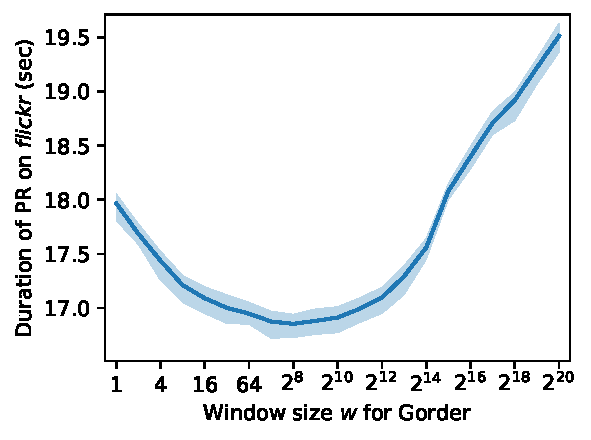
\includegraphics[width=.6\linewidth]{img/tune_w.pdf}
    \caption{\textbf{Tuning window size.} Versions of Gorder obtained for window sizes ranging from $w=1$ to $w=2^{20}\simeq 10^6$ are tested in PageRank over \textit{flickr} (with $n\simeq 2\cdot 10^6$ nodes). Median and 90\% confidence interval are shown for 100 repetitions. The plateau from $w=64$ to $w=2^{11}= 2048$ gives better results than $w=5$. This figure can be compared to Figure~8 in~\cite{gorder}; note that the absolute \runtime s are different because of hardware differences.
    }\label{img-tune-w}
\end{figure}

The choice of a small $w$ is yet relevant because of two other factors: first, the computation of Gorder is faster when the window is narrow, because a candidate node has to compute its proximity score $S$ with all the nodes of the window. Second, the authors of the original paper show that their heuristic is a $\frac{1}{2w}$-approximation of the optimal score: reducing $w$ makes this bound tighter.
%

Considering all these remarks and for the purpose of replication, we also use $w=5$ in the following experiments.



\section{Results} \label{results}

\subsection{Implementation hardware}
To deal with bigger datasets and ensure stability, we run the experiments on an isolated cluster (SGI UV2000 Intel Xeon E5-4650L @2.6 GHz, 128GB RAM). Each processor has three levels of cache of respective size 32kB, 256kB and 20MB.
%laptop (Intel Core i7-10810U @1.1GHz, 32GB RAM, Linux 5.4, Ubuntu 20.04.1, compiler GCC 9.3.0)
%a server (Intel Xeon Silver @2.40GHz, 256GB RAM, Linux 4.18, CentOS 8, GCC 8.3.1). 

The hardware used in~\cite{gorder} has similar cache and RAM storage but higher clock frequency, which can explain the differences in \runtime\ (in addition to programming techniques and optimisation). Note however that these differences should not modify the relative performance of different orderings.

\subsection{Ordering time}
Computing an ordering on a large network can be a long process, and some of the ordering methods have limited scalability. As mentioned above, Metis has been removed from the experiments for this reason.
%
Table~\ref{table-order-time} reports the duration of the ordering processes. For datasets under a hundred million edges, they can all be computed in a couple of minutes at most, with DegSort and ChDFS orderings requiring less than a second.


When the number of edges rises however, the computation takes hours for MinLA, MinLogA, and Gorder. In the case of MinLA and MinLogA, the number of steps is chosen arbitrarily as described in Section~\ref{orders}. The process could thus be interrupted earlier, at the cost of a less efficient resulting ordering.
%
As for Gorder, we can see that it does not scale linearly: the edges processed per second decrease from 380k for \textit{pokec} to 60k for \textit{sdarc}, which requires an almost 9-hour-long computation. Using a smaller window size accelerates the process but slightly worsens the resulting ordering, as seen in Figure~\ref{img-tune-w}.

\begin{table}[h]
\centering
\begin{tabular}{r||c|c|c|c|c|c|c|c}
  %\hline
& \textit{pokec} & \textit{flickr} & \textit{livejournal} & \textit{wiki} & \textit{gplus} & \textit{pldarc} & \textit{twitter} & \textit{sdarc}\\ 
  \hline%\hline
MinLA & 28 & 27 & 92 & 441 & 539 & 579 & \textbf{2956} & \textbf{4884}\\
MinLogA & 89 & 64 & 217 & \textbf{2169} & 1662 & \textbf{2258} & \textbf{10245} & \textbf{17168}\\
RCM & 3 & 5 & 10 & 60 & 49 & 63 & 158 & 406\\
DegSort & 0.8 & 0.4 & 1 & 5 & 9 & 14 & 30 & 85\\
ChDFS & 1 & 0.8 & 1 & 3 & 8 & 10 & 54 & 76\\
SlashBurn & 3 & 9 & 16 & 37 & 90 & 189 & 633 & 1066\\
LDG & 6 & 7 & 13 & 68 & 101 & 144 & 673 & 798\\
Gorder \footnotesize{$w$=$5$} & 79 & 110 & 118 & 988 & \textbf{3324} & \textbf{8783} & \textbf{25475} & \textbf{32488} \\
\hline
  Edges \footnotesize{$m$} & 31M & 33M & 69M & 437M & 463M & 623M & 1.47G & 1.94G
\end{tabular}
\caption{\textbf{Graph ordering time.} We indicate the time to compute each ordering in seconds (in bold font when above 30 minutes). We also indicate the number of edges for each dataset to help evaluating the scalability of a method. Comparing to Table~9 in~\cite{gorder} is possible for RCM, DegSort, ChDFS and Gorder because the implementations are alike: it shows that our hardware is 2 to 5 times slower than in~\cite{gorder}. For the other orderings, the implementations are likely too different to be compared.}\label{table-order-time}
\end{table}

%%%%%%%%%%%%
\begin{figure}%\newgeometry{left=10mm, right=10mm} 
    \begin{adjustwidth}{-25mm}{-15mm}
    \centering 
    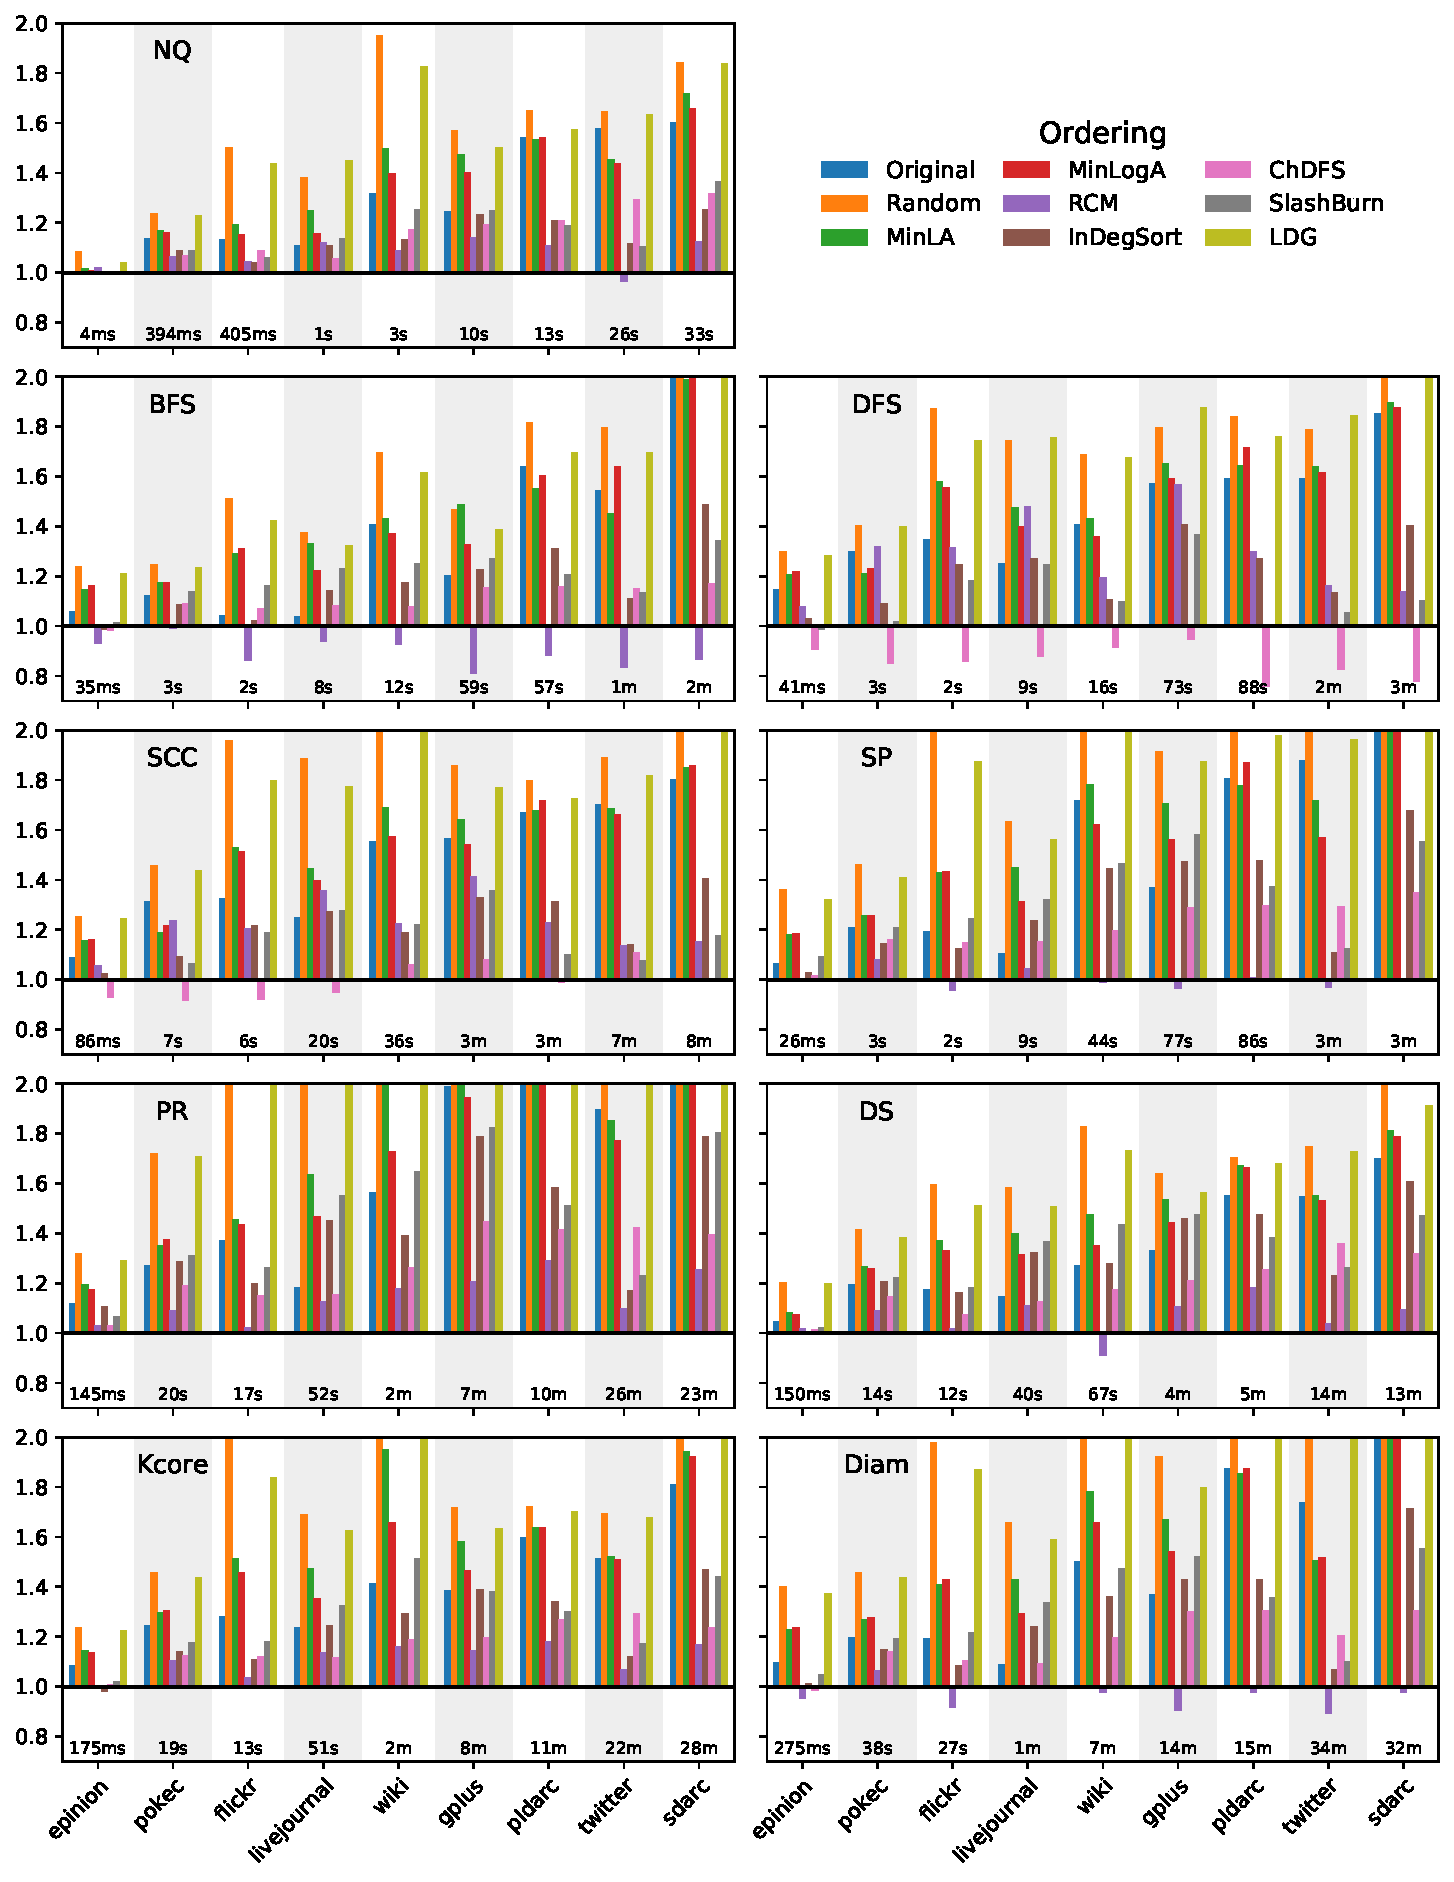
\includegraphics[width=\linewidth]{img/img-speedup.pdf}
    \caption{\textbf{Speedup of Gorder.} For each algorithm and each dataset, we display the absolute runtime for Gorder. Bars represent the relative time of all other orderings compared to this reference. For readability, the y-axis is cut above factor~2, but values go as high as 3.7. This figure can be compared to Figure~9 in~\cite{gorder}. Another visualisation is show in supplementary figure~\ref{img-speedup-grouped}.}\label{img-speedup}
    \end{adjustwidth}
\end{figure}%\restoregeometry

\subsection{Running time}
%
The main purpose of~\cite{gorder} is to measure if the node orderings listed above allow for faster execution of standard graph algorithms.
%
We compare in Figure~\ref{img-speedup} the performances of all the orderings to Gorder. The results are reported for each dataset and algorithm in the same way as Figure~9 of the original paper.
%
We also propose in supplementary figure~\ref{img-speedup-grouped} another visualisation of the same results but grouped by ordering instead of dataset, which emphasises the overall performance of an ordering method.


A first few observations can be made from the raw results of the experiments.
%
As in~\cite{gorder}, we observe that Gorder almost always leads to the fastest execution times.
%
The speed-up factor reaches up to 2.5 compared to default for Diameter on \textit{sdarc} and 3.7 compared to random for PageRank on \textit{wiki}, but for the sake of clarity we limit the y-axis of Figure~\ref{img-speedup} to a factor~2.

To help making sense of the results, we propose an aggregated visualisation in Figure~\ref{img-ranking}, where each ordering is ranked according to its performance in comparison to the other orderings through the 81 series of experiments reported in Figure~\ref{img-speedup}. It shows in particular that Gorder is the best ordering method in half of the experiments, and second-best in most other cases. 

Below, we comment on the performances of the different ordering methods under examination.




\subsubsection{Original ordering}
The experiments show that the default ordering performs better than more elaborate methods such as MinLA or MinLogA, which have a high computation overhead as shown in Table~\ref{table-order-time}. It was also observed in~\cite{gorder}.
%
This indicates that the way in which datasets are constructed tends to give close indices to nodes that are in the same neighbourhood. 
%
In a web graph for instance, if webpages are listed alphabetically by URL, it is likely that two consecutive nodes have a hyperlink between them since they belong to the same website.


\subsubsection{Poorly performing orderings}
The random ordering is always the worst performer except for 6 experiments where it is second-worst. It is not surprising as any other ordering tends to bring neighbouring nodes together, which should improve the algorithm \runtime.
%
Note however that LDG performs only slightly better than random, and that it is almost always the slowest in~\cite{gorder} too. In a quarter of the experiments, it is more than twice as slow as Gorder. These poor results lead to think that either its parameter (the size of bins $k=64$) is not optimal, or that its quality function is not highly correlated to cache efficiency.
%
MinLA and MinLogA are always faster than LDG but, except for \textit{twitter} dataset, they are slower than the original ordering. As reported in Figure~\ref{img-tune-sa}, we could not find any parameters with better results than local search, which is not ideal when the problem has local minima.


\subsubsection{Degree-based orderings}
%
Both InDegSort and SlashBurn use the degree of nodes as their main criterion. The experiments show that they outperform the default orderings, especially for larger datasets. For some algorithms such as BFS or NQ, they are less than 20\% slower than Gorder. This indicates that cache misses are reduced when nodes of similar degree are copied together on a cache line. 
The original paper found similar results, though their implementation of SlashBurn did not perform as well; the different version that we use here (see Section~\ref{orders}) may be responsible for this discrepancy. 


\subsubsection{Orderings outperforming Gorder on specific algorithms}
%
We also notice that some orderings perform particularly well on specific algorithms, even outperforming Gorder.
The ChDFS ordering is the most efficient for DFS algorithm on all datasets. This is due to the close relation between these two processes: the algorithm explores the graph in the exact same way as the ordering is created.
%
Likewise, RCM is a variation of a BFS that takes node degrees into account and it is the most efficient ordering for BFS algorithm.

Both also outperform Gorder for algorithms that are not as visibly related: ChDFS is up to 10\% more efficient for SCC on smaller datasets, and RCM is the most efficient for Diameter and SP.
More generally, Figure~\ref{img-ranking} shows that these two orders are among the three fastest ones in 75\% of the experiments. The original paper has different results on that matter: RCM and ChDFS are the best alternatives as well, but they are always 10 to 20\% slower than Gorder. 


\subsection{Comparison to the original paper}
Our purpose here is to detect if there are significant discrepancies in performance between the original paper and our replication study.

Figure~\ref{img-ranking} presents an aggregate view of the results grouped by ordering method.
%
For each series of experiments (\textit{i.e.} a given algorithm applied to a given dataset), we rank ordering methods from best to worst performance.
%
The figures report how many times each ordering has been ranked in each position. For instance Gorder is ranked first in 40 of our 81 replication series.


%%%%%%%%%%%%%
\begin{figure}[htb]
\centering 
\begin{subfigure}{.48\textwidth}
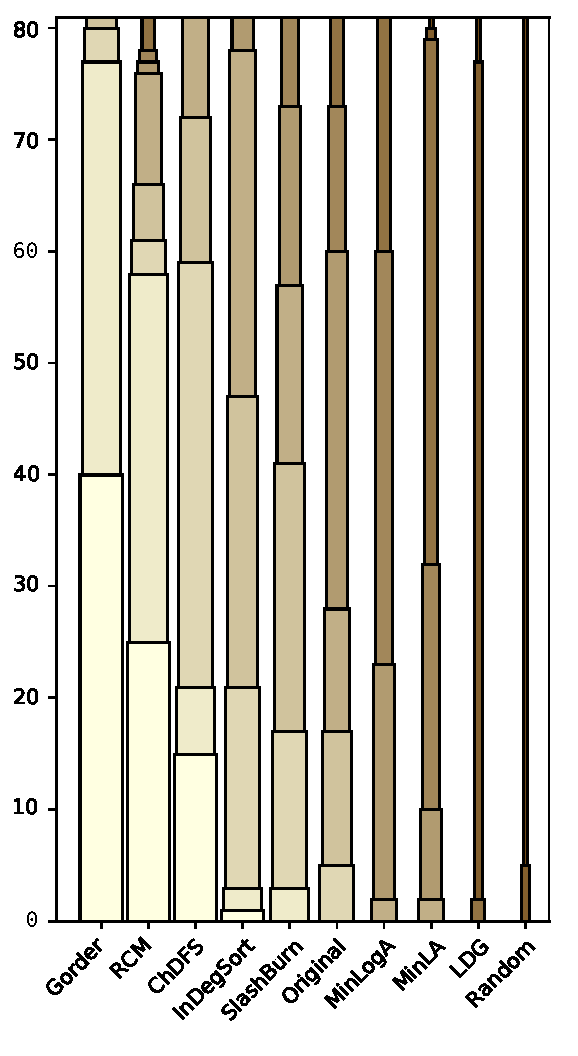
\includegraphics[width=\linewidth]{img/img-ranking_vert.pdf}
\caption{\textbf{Rankings in our 81 experiments} (9 algorithms times 9 datasets). Random ordering was added and Metis was ignored. }\label{img-ranking-fab}
\end{subfigure}
\hspace{.02\textwidth}
\begin{subfigure}{.48\textwidth}
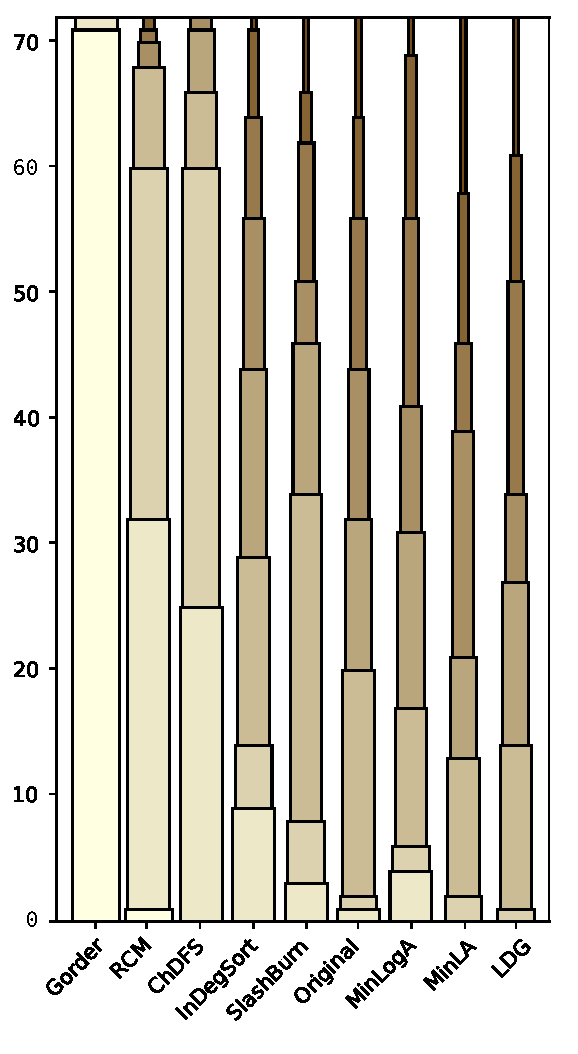
\includegraphics[width=\linewidth]{img/img-ranking-hao_vert.pdf}
\caption{\textbf{Rankings in \cite{gorder}} (72 experiments as \textit{epinion} is omitted). Rankings are inferred from Figure~9 of~\cite{gorder}: values above the factor 1.5 limit are considered equal.}\label{img-ranking-hao}
\end{subfigure}
\caption{\textbf{Rankings of ordering methods.} For each series of experiments, we rank the \runtime\ performance of the orderings. This figure shows how many times an ordering ranks best (thickest, lightest bar), second-best, \ldots, to worst (thinnest, darkest bar).}
\label{img-ranking}
\end{figure}
%%%%%%%%%%%%%




\subsubsection{Results for Gorder}
In both the original study and our replication, Gorder ranks first overall. This shows that this ordering is the best choice overall. However, our study shows that Gorder is outperformed by different orderings in half of the experiments, while it is only outranked once in the original paper. Figure~\ref{img-ranking-hao} thus leads us to think of Gorder as the perfect choice whereas Figure~\ref{img-ranking-fab} establishes RCM and ChDFS as relevant challengers, with 24 and 16 first places respectively.
%
This difference between the two papers is probably due to implementations: in our replication, ChDFS uses exactly the DFS algorithm. In particular, the nodes are visited in the same order, which leads to a quick execution of DFS. The original paper likely prevents this mechanism, for instance by shuffling the nodes at each step of the search.

\subsubsection{Ranking of other orders}
The three best orderings are evidently the same in both studies, but there are some nuances for the other ones. First, this visualisation does not always allow for exact ranking: in Figure~\ref{img-ranking-hao}, InDegSort has more second and third places than SlashBurn but fewer fourth and fifth places. There is no obvious way of deciding which is better, while Figure~\ref{img-ranking-fab} clearly indicates InDegSort. The same issue happens between Original and MinLogA: we can say that their rank in~\cite{gorder} is equal.

The last nuance comes for the slowest orderings: in our study, LDG is only better than Random while MinLA competes with MinLogA and Original. In~\cite{gorder} on the other hand, LDG is better than MinLA overall. Still, the limit at factor 1.5 makes the ranking unreliable for slowest orderings which can explain this difference.

In the end, both studies rank the orderings in a very similar way.

\subsubsection{Limits of visualisation}
The aggregate view of Figure~\ref{img-ranking} induces several approximations. First of all, there are 72 experiments in the original study and 81 experiments in ours, which adds \textit{epinion} dataset. This extra dataset is much smaller than the others and all its results in Figure~\ref{img-speedup} range in a 40\% factor, to be compared with more than 200\% for the biggest datasets. Yet, the ranking of ordering methods on \textit{epinion} is consistent with other datasets.

The original study does not test random orderings. This does not disturb the results as this method ranks last in most experiments. Similarly, our study omits Metis so we ignore it in Figure~\ref{img-ranking-hao} as well.
%
Moreover, the original paper hides precise information when a \runtime\ exceeds 1.5 times the \runtime\ of Gorder. We consider that all orderings above this bound are equal.

The main issue is that this visualisation only shows the rank and hides the extent of \runtime\ variations. This information is only visible in Figure~\ref{img-speedup}, where a rift separates two categories: faster orders with Gorder, RCM, ChDFS, InDegSort and SlashBurn, from slower orders with the other ones. However, Figure~\ref{img-ranking} is useful to grade ordering methods. If original ordering is taken as a limit between faster and slower orders, we find the same gap again.

\subsection{Cache miss}

A cache miss is a state of an execution when the data requested by the processor is not found in the cache memory. The program has to fetch the data in further cache levels or in main memory, which causes delays.
%
Gorder capitalises on the intuition that if we cluster nodes that are frequently accessed together, higher levels of cache will hold more relevant data and thus make algorithms run faster.


To prove that Gorder speedup is due to cache optimisation, we compute the proportion of the total computation time spent in data retrieval. 
%
We use Unix \textit{perftools} with the wrapper \textit{ocperf}. 
It provides various hardware metrics such as the number of CPU cycles, branch predictions, cache misses\ldots
%
\footnote{See \url{https://perf.wiki.kernel.org}. We select the following counters:
the total time \textit{task-clock}, \textit{cpu-cycles}, \textit{L1-dcache-loads} and \textit{L1-load-misses} to measure the efficiency of the first layer of data cache (we are not interested in instruction cache here), \textit{LLC-loads} and \textit{LLC-load-misses} to measure the efficiency of the last cache layer, and metrics specifically designed to measure the impact of cache misses such as \textit{cycles-l1d-pending} or \textit{cycles-l3-miss} in the cycle-activity category.}
%
Depending on the machine architecture, different metrics are available.
%
\begin{table}[bt]
\begin{subtable}[t]{\linewidth}
\centering
\begin{tabular}{r||c|c|c|c|c}
Order & L1-ref (10$^9$) & L1-mr & L3-ref (10$^9$) & L3-r & Cache-mr \\ \hline
Original & 29 & 15.9 \% & 2.8 & 9.8 \% & 2.5 \% \\
Random & 30 & 20.2 \% & 4.1 & 13.6 \% & 3.6 \% \\
MinLA & 29 & 16.2 \% & 3.3 & 11.4 \% & 2.5 \% \\
MinLogA & 28 & 15.9 \% & 3.1 & 10.7 \% & 2.5 \% \\
RCM & 30 & 11.5 \% & 1.8 & 5.9 \% & \textbf{1.6 \%} \\
InDegSort & 28 & 14.7 \% & 2.5 & 9.1 \% & 2.2 \% \\
ChDFS & 29 & 12.8 \% & 2.1 & 7.2 \% & 1.8 \% \\
SlashBurn & 28 & 14.8 \% & 2.6 & 9.3 \% & 2.2 \% \\
LDG & 30 & 19.2 \% & 3.7 & 12.4 \% & 3.2 \% \\
Gorder & 28 & \textbf{10.3 \%} & \textbf{1.4} & \textbf{5.0 \%} & 1.7 \% \\
\end{tabular}
\caption{On \textit{flickr} dataset.}
\label{table-cache-flickr}\end{subtable}

\begin{subtable}[t]{\linewidth}
\centering
\begin{tabular}{r||c|c|c|c|c}
Order & L1-ref (10$^9$) & L1-mr & L3-ref (10$^9$) & L3-r & Cache-mr \\ \hline
Original & 1885 & 19.0 \% & 303 & 16.0 \% & 6.8 \% \\
Random & 1886 & 23.4 \% & 397 & 21.0 \% & 9.0 \% \\
MinLA & 1893 & 21.2 \% & 341 & 18.0 \% & 7.1 \% \\
MinLogA & 1885 & 20.7 \% & 330 & 17.5 \% & 6.9 \% \\
RCM & 1885 & 11.0 \% & 139 & 7.4 \% & 3.7 \% \\
InDegSort & 1779 & 15.0 \% & 198 & 11.1 \% & 6.0 \% \\
ChDFS & 1863 & 11.8 \% & 153 & 8.2 \% & 4.3 \% \\
SlashBurn & 1784 & 15.3 \% & 203 & 11.4 \% & 6.0 \% \\
LDG & 1886 & 22.9 \% & 387 & 20.5 \% & 8.8 \% \\
Gorder & 1816 & \textbf{9.3} \% & \textbf{104} & \textbf{5.7 \%} & \textbf{3.1 \%} \\
\end{tabular}
\caption{On \textit{sdarc} dataset.}
\label{table-cache-sdarc}\end{subtable}

\caption{
    \textbf{Cache statistics measured for PageRank algorithm.} L1-ref (references): number of times a piece of data was required by the processor and searched in level 1 of cache. L1-mr (miss-rate): proportion of data that was not found in L1. L3-ref: number of references to the third (lowest) level of cache after data was not found in levels 1 and 2. L3-r (ratio): proportion of data that was not found in L1 nor L2, then searched in L3. Cache-mr: proportion of data that was not found in cache (L1, L2 or L3) and had to be retrieved in main memory. Compare to Tables~3 and~4 in~\cite{gorder}.
}
\label{table-cache}
\end{table}


Table~\ref{table-cache}, just like the Tables~3 and~4 of the original paper, shows the cache-miss rates at different levels. The first column is the total number of L1-references which is the number of times a piece of data was required by the processor. A proportion of this data is not found (second column) and requested in intermediate levels of cache, until reaching L3 (third and fourth columns). The remaining data (last column) has to be retrieved in main memory. Note that each further level of cache roughly implies an additional factor 4 latency. 

We observe that first-level cache references are similar for all orderings: the algorithms run in the exact same way so they need to access the same amount of data, regardless of the arrangement of nodes. However, the miss-rate in L1 reveals important variations: with Gorder, only 10\% of the data is not directly available in L1, while it reaches 20\% with Random or LDG orders. 
%
The percentage of data requested in L3 is even more scattered, from 5\% with Gorder to 20\% with Random or LDG on \textit{sdarc}.
%
Finally, all the orderings have a low cache-miss rate (between 1.6 and 3.6\%) on \textit{flickr} and RCM has the smallest. The gap is more striking on \textit{sdarc} where Random and LDG have 9\% of cache-miss, three times as much as Gorder. This ratio is the proportion of data that had to be retrieved in main memory (RAM), which is about 60 times slower than the L1 cache\footnote{At 4GHz, a cycle is $1c=1/(4\cdot 10^9)s=0.25ns$, so latency is $4c=1ns$ for L1 and $42c+51ns\simeq 62ns$ for RAM. Values are taken from \url{https://www.7-cpu.com/cpu/Skylake.html}.}.

In general, the ranking for cache-miss rates matches the ranking for \runtime\ shown in Figure~\ref{img-ranking-fab}. Gorder has the best results and RCM and ChDFS are close behind. MinLA, MinLogA and Original orders have high cache-miss rates for all levels. This shows that the speedup is indeed due to cache-miss reduction.
%
When compared to Original order, Gorder reduces cache-miss rates to speed up the algorithms. Figure~\ref{img-cache} shows that the total \runtime\ is reduced by 15 to 50\% on \textit{sdarc}, but the CPU execution time is almost identical: it is the factor 3 reduction on cache stall that makes the algorithm faster. 






\section{Discussion}\label{discussion}

Our experiments replicate the ones proposed in~\cite{gorder} but some aspects are not discussed in sufficient detail in the original paper to allow for immediate replication.
%
For instance, the algorithms NQ and DS only have a succinct description, which may explain why their performances reported in our Figure~\ref{img-cache} do not align perfectly with Figure~1 of \cite{gorder}. 
Similarly, we were not able to tune the simulated annealing procedure correctly, which questions the relevance of our experiments with MinLA and MinLogA.
%
Nonetheless, most of these technical issues have been solved or circumvented thanks to the answers of Hao Wei to our questions.

Above all, this study replicates the main observation of the original paper: Gorder reduces cache latency significantly and is the best performer among all the ordering methods under study, as shown in Figure~\ref{img-ranking}. Its consistent efficiency on all algorithms and datasets suggests that it could speed up other graph algorithms as well.

The only important difference with the original paper is that RCM and ChDFS follow closely behind Gorder and even outperform it in half of the experiments. They are based on straightforward graph searches, which are simple to program and very quick to execute, as reported in Table~\ref{table-order-time}.
%
On the other hand, computing Gorder requires a complex procedure and a lot of time. It has been pointed out in~\cite{overhead} that this high overhead time can only be amortised if algorithms are run thousands of times. In the case where networks evolve and require constant recomputation of the node ordering, Gorder needs to be adapted to integrate the modifications without running the whole process again. A parallel version of Gorder could reduce this problem.

Beyond algorithm speed-up, the contribution of Hao Wei \textit{et al.} is an efficient framework that could be applied for other purposes. For example, graph compression also benefits from orderings that cluster nodes with high proximity~\cite{boldiv}. Gorder could be an input for such existing methods. It would also be interesting to investigate how different types of real-world datasets~\cite{milo} behave when a new ordering is applied. 




\section{Conclusion}

The replication of paper \cite{gorder} shows that Gorder is an efficient cache optimisation for various standard algorithms.
%, though some orders are still faster for specific algorithms.
We confirm its superiority for networks ranging from 30 million to 2 billion edges, and the hardware measurement tools prove that this is due to reduced cache stall. However, orders such as DFS are among the best performers, and they are much simpler to design. Indeed, the computation of Gorder does not scale linearly, which makes it very time-consuming for bigger graphs. It is then a matter of balance between this long overhead time and the substantial speedup for subsequent graph algorithms.

%%%%%%%%%%%%
% \newpage
%%%%%%%%%%%%

\subsection*{Acknowledgements}

We warmly thank Hao Wei for replying to our questions about the original paper, which settled several technical hesitations relative to the implementation.

This work is funded by the ANR (French National Agency of Research) partly by the \href{http://bit.ly/LiMass}{LiMass JCJC project} (under grant ANR-19-CE23-0010) and partly by the \href{http://fit.complexnetworks.fr}{ANR FiT LabCom}.

